% ch11: 原文 GLDraft_D.tex 行 2441–2842；§7.3–7.7
% 只译散文（标题、正文、图题、脚注）；公式、\label、\ref、\eqref、\cite、图文件名保持不变。

\subsection{从角到态} \label{fcs}

现在考虑一个条带（strip）：两端分别放置 $\B_{\cc}$ 与 $\bar \B_{\cc}$，底边则由另一张膜 $\B$ 设定边界条件（图 \ref{example6}）。在“角”处，我们刚刚描述的构造给出两个手征代数（chiral algebra）$\V$ 与 $\bar \V$。在角上作适当的算符插入后，条带上的路径积分给出一个（可能只作为分布定义的）态
\be\label{chidef}
\chi = \left|O_1(z_1) \cdots O_n(z_n) \bar O_{n+1}(\bar z_{n+1}) \cdots \bar O_{n+\bar n}(\bar z_{n+ \bar n})\right\rangle
\ee
它属于通常的希尔伯特空间 $\H=\Hom(\b\B_\cc,\B_\cc)$。一个重要特例是：两个角上的手征代数 $\V$ 与 $\bar\V$ 互为复共轭；不过我们并不限于这一情形。位于不同角上的算符之间不可能出现 OPE 奇异性，因此 $\bar \B_{\cc}$ 角上的 $\bar O_j(\bar z_j)$ 不影响 $O_i(z_i)$ 的 Ward 恒等式，反之亦然。

我们也可以考虑 $\chi$ 与一个检验态 $\Psi \in {\cal H}$ 的配对。所得内积一般而言可能并不良定义；但只要 $\Psi$ 足够好，它就是良定义的——例如 $\Psi$ 由条带顶端一张具有紧支撑（compact support）的膜按类似方式产生（图 \ref{example6}(c)）。若对任意算符插入的选取该内积都良定义，它就给出 $C$ 上的一族关联函数
\be
\langle \Psi| O_1(z_1) \cdots O_n(z_n) \bar O_{n+1}(\bar z_{n+1}) \cdots \bar O_{n+\bar n}(\bar z_{n+ \bar n}) \rangle
\ee
这些关联函数满足 ${\cal V}$ 与 $\bar {\cal V}$ 的 Ward 恒等式。

用边界线缺陷（boundary line defect）装饰的半 BPS（half-BPS）边界条件会产生更大的一族态
\be
\left|\prod_i O_i(z_i) \prod_j \bar O_{j}(\bar z_{j}) \prod_k O_{\ell_k,k}(p_k) \bar O_{\ell_k,k}(\bar p_k) \right\rangle,
\ee 
其角数据还包含边界线缺陷的端点。

本节余下部分将针对半 BPS 边界条件的几个基本例子，把这些结构具体写出来。

\subsection{Dirichlet 边界条件}\label{Dbc}
四维半 BPS 的 Dirichlet 边界条件把规范联络 $A$ 固定为在边界上为零——更一般地，固定为在边界上取某个指定值——并以超对称的方式延拓到其余场。特别地，六个标量场中有三个满足 Dirichlet 边界条件，另外三个（其中包括二维 $\sigma$-模型的希格斯场 $\phi$）满足 Neumann 边界条件。

从定义在 $\partial M$ 的一部分 $N$ 上的辅助 $\varphi \cF$ 理论来看，半 BPS Dirichlet 边界条件与变形 Neumann 边界条件之间的交汇，由沿 $\partial N$ 加在场 $\cA_{\bar z}$ 上的 Dirichlet 边界条件表示。规范变换被限制为在边界上平凡；否则就不可能指定 $\cA_{\bar z}$ 沿边界的值。对 $\cA_{\bar z}$ 的共轭 $\varphi=\varphi_z\d z$，我们不加任何边界条件。

由于规范变换被约束为沿 $\partial N$ 平凡，$\partial N$ 上（也就是交汇处）的局部算符不必是规范不变的。取而代之，存在一个作用在 $\partial N$ 上算符的整体 $G$ 对称性\footnote{\label{defglobal} 元素 $g\in G$ 给出的整体对称变换，是一个规范变换 $g(x):N\to G$，其在 $\partial N$ 上的限制为常数，$g(x)|_{\partial N}=g$。它保持条件 $\cA_{\bar z}|_{\partial N}=0$，因此是该边界条件下所定义理论的对称性。常数 $g$ 如何在 $N$ 的内部延拓为一个规范变换并不重要：任意两种选取之差是一个在边界上平凡、且对物理可观测量作用平凡的规范变换。}；$\cA$ 的边界值 $a$ 可以解释为该整体 $G$ 对称性的背景联络。在四维设置中，$G$ 对称性作用在整个半 BPS Dirichlet 边界条件上；但在 $A$-扭化中，$N$ 的内点处没有任何局部算符可供它作用。整体对称性只作用在交汇处的算符上。

标量场 $\varphi$ 是交汇处的一个合法局部算符，它等同于辅助 $\varphi \cF$ 理论中的同一算符。在 $A$-扭化理论中，算符 $\varphi_z$ 实际上就是相应于边界 $G$ 对称性的守恒流。导出这一结果的一种方式如下。若在“自由”边界条件下变分作用量 $I_{\varphi\cF}=\int_N \Tr\,\varphi_z F_{t\bar z}\d t \d^2z$，就会发现 $I_{\varphi \cF}$ 的变分含一个边界项 $\int_{\partial N} \Tr\,\varphi_z\delta A_{\bar z}$，因此 Euler–Lagrange 方程中包含边界条件 $\varphi_z|_{\partial N}=0$，而对 $A_{\bar z}$ 不加限制。反之，若希望边界条件为 $A_{\bar z}=a_{\bar z}$（其中 $a$ 是 $C$ 上某个指定的联络），可以在作用量上加一个边界项，使总作用量成为
\be\label{fullact} I'_{\varphi\cF}=I_{\varphi\cF}-\int_{\partial N}\Tr\,\varphi_z(A_{\bar z}-a_{\bar z}).\ee
此时 Euler–Lagrange 方程给出的边界条件是 $(A_{\bar z}-a_{\bar z})|_{\partial N}=0$，对 $\varphi$ 不加约束。但这时流为 $J_z=\partial I'_{\varphi\cF}/\partial a_{\bar z}=\varphi_z$，与断言相符。

如第 \ref{ACP} 节与 \cite{Gaiotto:2017euk} 所解释的，在把这一问题推广到一般 $\Psi$ 的情形时，$J_z$ 是 Kac–Moody 流这一点在经典层面即可看出；但要证明 level 是 $\Psi-h$ 而非 $\Psi$，还需要一个与我们即将描述的类似的三维单圈计算。当 $\Psi=0$ 时，Kac–Moody level 完全来自单圈计算。所需的计算可以借助一个简单的捷径非常容易地完成，这个捷径在任何维数的规范场论中都有类似物。我们把 $\varphi\cF$ 理论放在平板（slab）$I\times C$ 上，其中 $I$ 是区间 $[0,L]$，两端具有相同的 Dirichlet 边界条件。反常总可以由理论的低能极限算出，因此在此情形可以丢掉沿 $I$ 非常数的模式，约化为一个纯二维理论。这等价于取朴素的 $L\to 0$ 极限。所得的二维理论具有作用量
\be\label{belaction}
\int \Tr \, \varphi_z D_{\bar z} \cA_t\ee
它是场为 $\varphi_z$ 与 $\cA_t$（此时只依赖 $z$ 与 $\bar z$，不依赖 $t$）、自旋分别为 1 与 0、取值于伴随表示的玻色型 $\beta \gamma$ 系统。类似的、取值于伴随表示的费米型手征 $bc$ 系统具有反常系数 $2h$，因此玻色型 $\beta\gamma$ 系统的反常为 $-2h$。在平板 $I\times C$ 上的规范场论中，由于体理论没有反常，反常局域在平板的两个边界上。由对称性，一半反常来自平板的一端，另一半来自另一端，故任一端的反常系数为 $-h$。这个 level 取值具有非常特殊的性质，我们马上就会回顾。Kac–Moody level 的取值 $-h$ 常被称为临界 level（critical level），记作 $\kappa_c$。\zy{译者按：临界 level $\kappa_c=-h$ 的特殊性在于 Sugawara 构造 $T(z)=\frac{1}{\kappa+h}S_2(z)$ 的分母为零：通常的应力张量退化，$S_2$ 与所有 Kac–Moody 流的 OPE 变为正则，从而成为中心元。标准处理见 P. Di Francesco, P. Mathieu and D. Sénéchal, \emph{Conformal Field Theory}, Springer, 1997, §15。}

下面来确定 $\varphi\cF$ 规范场论的体局部算符 ${\cal P}[\varphi](z)$ 在 ${\cal V}$ 中的像。朴素地看，像就是 ${\cal P}[J](z)$。然而，由于 $J_z$ 与自身的 OPE 奇异性，这一表达式并不良定义。我们可以用点分裂（point splitting）来正规化它，小心地减去奇异项。这其实是二维共形场论中一个熟悉的练习。

最简单的例子是二次哈密顿量 $\Tr\, \varphi_z^2$ 的像。该算符的正规化版本就是 Sugawara 算符 $S_2(z)$。回忆一下：对一般的 level $\kappa$，Sugawara 算符与应力张量成正比，$T(z) = \frac{1}{\kappa + h} S_2(z)$。特别地，$S_2(z)$ 的 OPE 的奇异部分
\begin{equation}
S_2(z) J(w) \sim (\kappa + h)\frac{J(w)}{(z-w)^2} + (\kappa + h) \frac{D_w J(w)}{z-w} + \cdots
\end{equation}
正比于经临界平移后的 level $\kappa+h$。当 $\kappa=\kappa_c=-h$ 时，$S_2(z)$ 与 Kac–Moody 流的 OPE 非奇异，也就是说它是中心元。这正是我们期望 $\Tr \varphi_z^2$ 在 ${\cal V}$ 中的像所具有的性质，并且在具有相同标度维数的算符中完全刻画了它。因此 $S_2(z)$ 对应二次的 Hitchin 哈密顿量。

更高次哈密顿量的正规化要费力一些，但我们可以援引一个一般定理 \cite{BD}：$G$ 的临界 Kac–Moody 代数的中心由一组中心元 $S_{\P}(z)$ 生成，这些中心元正是 ${\cal P}[J](z)$ 的正规化。作为代数，临界 Kac–Moody 代数的中心同构于朗兰兹对偶群 $G^\vee$ 的 oper 流形 $L_\op$ 上全纯函数的空间。由此我们断定：$S_{\P}(z)$ 就是三维算符 ${\cal P}[\varphi](z)$ 在交汇处的像；而通过 $S$-对偶，这些三维算符又被等同于 $L_\op$ 上全纯函数代数的生成元。

Dirichlet 边界上存在整体 $G$ 对称性，这为全纯-拓扑（holomorphic–topological）BAA 型膜的构造增添了一个要素。如前所述，我们可以把 Dirichlet 边界条件推广：不再把联络的边界值取为零，而取 $C$ 上任意固定的联络 $a$。这样就得到一整族 BAA 型膜 $\mathrm{Dir}(a)$，由背景 $G$ 联络 $a$ 的选取参数化。在 $A$-扭化理论中，系统只依赖 $\B_\cc$ 角上的 $a_{\bar z}$ 与 $\bar \B_\cc$ 角上的 $a_z$。这一依赖分别编码在 $\B_\cc$ 角的全纯流 $J_z$ 与 $\bar \B_\cc$ 角的反全纯流 $\bar J_{\bar z}$ 之中。\zy{译者按（无外部依据）：BAA 是 Kapustin–Witten 对膜型的记法：按复结构 $I,J,K$ 的顺序，该膜依次为 $B$-型、$A$-型、$A$-型，即 $(B,A,A)$ 型；本译本有时也直接写作“型 $(B,A,A)$ 的膜”。参见原文所引 Kapustin–Witten 的工作。}

在交汇处没有局部算符插入时，Dirichlet 边界条件于是定义了一族（分布意义的）态 $\Delta(a) \in \H$。在两个角上插入 Kac–Moody 流 $J_z(z_i)$ 或 $\bar J_{\bar z}(\bar z_j)$，就给出该态对背景联络的泛函导数
\be
\prod_i \frac{\delta}{\delta a_{\bar z}}(z_i) \prod_j \frac{\delta}{\delta a_{ z}}(\bar z_j) \Delta(a)
\ee 
这里对背景联络求泛函导数。
 
全纯与反全纯联络的 Kac–Moody 性质有一个重要推论：这两个流分别守恒。回忆带反常的守恒律：
\begin{align}
D_{\bar z} J_z &= - \frac{\kappa_c}{2 \pi} f_{z \bar z} \cr
D_z J_{\bar z} &= \frac{\kappa_c}{2 \pi} f_{z \bar z}
\end{align}
其中 $f$ 是 $a$ 的曲率。这些式子表明：在 $a$ 的无穷小复化规范变换下，态 $\Delta(a)$ 协变地、但带有反常地变换。精确到 $\lambda$ 的一阶，
\be 
\Delta(a_z + D_z \bar \lambda, a_{\bar z} + D_{\bar z} \lambda )=\left[1+\frac{\kappa_c}{2 \pi} \int_C \Tr\left(\bar \lambda - \lambda \right)f_{z \bar z}  \right] \Delta(a_z,a_{\bar z})
\ee
一个足够好的抽象态 $\Psi \in \H$ 与 $t=0$ 处的 Dirichlet 边界条件配对后，给出一个泛函 $\Psi(a)$；在 $a$ 的无穷小复化规范变换下，它作类似的变换：
\be \label{eq:cogauge}
\Psi(a_z + D_z \bar \lambda, a_{\bar z} + D_{\bar z} \lambda )=\left[1+\frac{\kappa_c}{2 \pi} \int_C \Tr\left(\bar \lambda - \lambda \right)f_{z \bar z}  \right] \Psi(a)
\ee  注意，$\Psi$ 在实规范变换下不变，后者对应 $\lambda=\bar\lambda$ 这一特例。$\Psi(a)$ 对 $a$ 的泛函导数给出临界 Kac–Moody 流与 $a$ 耦合的关联函数。

\subsection{联络与丛}\label{CB}

设 $a$ 是黎曼曲面 $C$ 上的联络，结构群为紧规范群 $G$。考虑一个函数 $\Psi(a)$，它不只在 $G$ 值规范变换下不变，而且在 $G_\C$ 值规范变换下不变；后者在无穷小层面作用为
\be\label{actfor}\delta a_{\bar z}=-D_{\bar z}\lambda, ~~\delta a_z=-D_z\bar\lambda. \ee
这样的函数决定 $\M(G,C)$ 上的一个函数，因为 $\M(G,C)$ 可以看作所有 $G$ 值联络构成的空间对复规范变换群的商。\footnote{这一描述略欠精确，因为要真正把 $\M(G,C)$ 实现为商，还需考虑稳定性方面的因素。但实际上并无困难：只要函数 $\Psi(A)$ 连续且在 $G_\C$ 值规范变换下不变，它就确实下降为 $\M(G,C)$ 上的函数。从所有联络的空间走到 $\M(G,C)$，需要丢掉那些定义不稳定全纯丛的联络，在半稳定者上强加一个等价关系，然后取商。连续且 $G_\C$ 不变的函数 $\Psi(a)$ 必定在该等价关系下不变。无论如何，对 $\lmark^2$ 理论而言，这些考虑都不重要。下一段也有类似的说明。}

反之，给定 $\M(G,C)$ 上的函数 $f$，要在联络空间上定义函数 $\Psi(a)$，只需规定：对给定的 $a$，$\Psi(a)$ 等于 $f$ 在 $\M(G,C)$ 中对应于全纯丛 $E\to C$ 的那一点处的值，而该丛由 $a$ 的 $(0,1)$ 部分决定。这样定义的函数 $\Psi(a)$ 自动在 $G_\C$ 值规范变换下不变。

$\M(G,C)$ 上的函数与 $G_\C$ 不变的联络函数之间的这一对应，可以推广到并不 $G_\C$ 不变、而是带反常地在 $G_\C$ 值规范变换下协变变换的函数 $\Psi(a)$。这些泛函可以等同于 $\M(G,C)$ 上某个线丛的截面。对我们最重要的情形是：$\Psi(a)$ 的全纯与反全纯反常系数均为 $\kappa_c=-h$，如式 (\ref{eq:cogauge}) 所示。此时该线丛实际上就是 $\M(G,C)$ 上的半密度丛，我们稍后会说明这一点。更一般地，若把 $\kappa_c$ 换成别的 level $\kappa$（全纯与反全纯两侧相同），则 $\Psi(a)$ 表示 $|K_{\M(G,C)}|^{\frac{\kappa}{\kappa_c}}$ 的截面。

\begin{yizhu}[译者按：为什么反常系数对应半密度]
$\M(G,C)$ 的辛体积元属于经典辛结构，但不属于 $A$-模型。原文的论证是：若物质泛函的反常为 $2\kappa_c$，则它与 level 为 $-2\kappa_c$ 的 Faddeev–Popov 鬼场系统相乘后总反常为零，BRST 流幂零，被积式与代表的选取无关，因而可在 $\M(G,C)$ 上积分——这就是“密度”。反常减半即得半密度，即 $|K_{\M(G,C)}|^{1/2}$ 的截面；一般 level $\kappa$ 则给出 $|K|^{\kappa/(2\kappa_c)}$（原文作 $\kappa/\kappa_c$，疑为笔误；两者在 $\kappa=\kappa_c$ 时一致）。原文借玻色弦中心荷 $c=26$ 的路径积分作类比，并指出这一对应最早由 Beilinson 与 Drinfeld 给出（见原文所引其著作）。
\end{yizhu}

要说明“以全纯与反全纯反常系数 $\kappa_c$ 变换的函数对应 $\M(G,C)$ 上的半密度”，有许多办法（这最早由 Beilinson 与 Drinfeld \cite{BD} 指出）。我们的做法是先说明：以反常系数 $2\kappa_c$ 变换的函数是 $\M(G,C)$ 上的密度。所谓 $\M(G,C)$ 上的密度，是指这样一种对象：它可以在 $\M(G,C)$ 上自然地积分，而不需要用到 $\M(G,C)$ 的任何结构，只用到它是联络空间对 $G_\C$ 值规范变换群的商这一事实。要判断 $\Psi(a)$ 属于哪一类可在 $\M(G,C)$ 上积分的对象，我们将使用一个与玻色弦路径积分之定义有些类似的构造。

考虑一个带联络 $a$ 的二维 $G$ 规范场论，它与某个物质系统耦合，后者具有 level 为 $(\kappa, \kappa)$ 的全纯与反全纯 Kac–Moody 对称性。由于该理论的路径积分在复化规范变换下形式不变，我们可以期望把路径积分规范固定为 $\M(G,C)$ 上的积分。为此需要一族规范固定条件。我们只需对 $\M(G,C)$ 中的每一点 $m$ 挑一个代表二维联络 $a[m, \bar m] = (a_z[\bar m], a_{\bar z}[m])$，并取规范 $a = a[m, \bar m]$。目标是把对 $a$ 的积分化为对 $m,\bar m$ 的积分。

我们按惯例为这一规范固定引入 Faddeev–Popov 鬼场（ghost）。具体地说，引入与复化规范参数 $\lambda$、$\bar \lambda$ 相应的伴随值鬼场 $c$、$\bar c$，以及与规范固定条件相应的伴随值 1-形式 $(b_z, \bar b_{\bar z})$。鬼场作用量为
\begin{equation}
\int\left( \Tr \,b_z D_{\bar z} c +  \Tr \,b_{\bar z} D_z c\right)\d^2z.
\end{equation}  
该鬼场系统具有全纯与反全纯 Kac–Moody 对称性，level 为 $(2h,2h)=(-2\kappa_c, -2\kappa_c)$。众所周知，BRST 流幂零，当且仅当物质加鬼场的总反常为零，即当且仅当 $\kappa - 2 \kappa_c=0$。

$\M(G,C)$ 上的被积表达式是借助 $b$ 的零模准备好的。若把物质配分函数记作 $\Psi(a)$，则规范固定后的路径积分成为
\begin{equation}
\int_{\M(G,C)} \Psi\left(a[m,\bar m]\right) \left\langle \prod_i \left[\int_C b_z \frac{\partial a_{\bar z}[m]}{\partial m_i} \d m_i \right] \left[\int_C b_{\bar z} \frac{\partial a_{z}[\bar m]}{\partial \bar m_i} \d \bar m_i \right] \right\rangle
\end{equation}   这里我们只是模仿了玻色弦与全纯、反全纯中心荷均为 $c=26$ 的共形场论耦合时路径积分的通常定义。由此可知：level 为 $2 \kappa_c$ 的规范协变泛函对应 $\M(G,C)$ 上的密度。

于是，如 (\ref{eq:cogauge}) 那样 level 为 $\kappa_c$ 的规范协变泛函对应 $\M(G,C)$ 上的半密度。在这一表述下，我们可以把希尔伯特空间的内积显式写出：
\begin{equation}\label{eq:innergauge}
\left( \Psi', \Psi \right) \equiv \int_{\M(G,C)} \overline{\Psi}'\left(a[m,\bar m]\right) \Psi\left(a[m,\bar m]\right) \left\langle \prod_i \left[\int_C b_z \frac{\partial a_{\bar z}[m]}{\partial m_i} \d m_i \right] \left[\int_C b_{\bar z} \frac{\partial a_{z}[\bar m]}{\partial \bar m_i} \d \bar m_i \right] \right\rangle
\end{equation}

现在，把一个（足够好的）态 $\Psi \in \H$ 联系到一个泛函 $\Psi(a)$，有两条途径：其一，把抽象态等同于 $\M(G,C)$ 上的半密度，再把它提升为联络的泛函；其二，把 $\Psi$ 与平移后的 Dirichlet 边界条件 $\mathrm{Dir}(a)$ 所产生的态 $\Delta(a)$ 作缩并。为说明这两种做法等价，可以这样论证。经典地看，BAA 型膜 $\mathrm{Dir}(a)$ 支撑在 $T^*\M(G,C)$ 中由 $a_{\bar z}$ 所定义丛 $E$ 处的纤维上。这是余法拉格朗日子流形的最简单类型，相应的态 $\Delta(a)$ 具有集中于 $E$ 处的 delta 函数支撑。因此配对 $ (\Delta(a), \Psi)$ 无非就是泛函 $\Psi$ 在联络 $a$ 处的取值。

作为最后一个练习，我们可以回到量子 Hitchin 哈密顿量的定义。我们希望导出一个公式，用与 $\Psi$ 相联系的泛函 $\Psi(a)$ 来表达哈密顿量作用于某个 $\Psi$ 后所得的泛函 $[\D_\P(z) \circ \Psi](a)$。考虑一个条带：左边界取 $\B_\cc$ 边界条件，底边取某个初始条件，它与角上的数据一起定义态 $\Psi$。（这一设置已示意于图 \ref{example6}(b)，其中条带底部的膜记作 $\B_F$。）按定义，泛函 $[\D_\P(z) \circ \Psi](a)$ 通过在左边界插入 $\P[\varphi_z]$ 并把它移到条带的左下角来计算。这样做时，$\P[\varphi_z]$ 被转换为手征代数的中心元 $S_{\P}(z)$，即 $J_z$ 及其导数的某个正规化多项式。反过来，$J_z$ 的插入可以换成对 $a_{\bar z}$ 的泛函导数。于是 $[\D_\P(z) \circ \Psi](a)$ 被表示为作用在 $\Psi(a)$ 上的某个微分算子 $\D^{(a)}_\P(z)$。算符 $\D^{(a)}_\P(z)$ 是 $\P\left[\frac{\delta}{\delta a_{\bar z}} \right]$ 的正规化。它把规范协变泛函映为规范协变泛函，恰恰是因为 $S_{\P}(z)$ 是中心元：$S_{\P}(z)$ 的插入不改变流的 Ward 恒等式，因而微分算子 ${\cal D}^{(a)}_{\P}(z)$ 与规范协变性约束 (\ref{eq:cogauge}) 对易。量子 Hitchin 哈密顿量在数学上正是这样定义的 \cite{BD}：它们刻画了临界 Kac–Moody 代数的共形块（conformal block）中插入一个 $S_{\P}(z)$ 的效果。

要用类似方式表述 Hecke 算符，还需讨论 Dirichlet 边界条件上的边界 't Hooft 算符及其在交汇处的端点。在辅助的三维视角下，边界 't Hooft 算符映为边界单极子算符。这类无序算符（disorder operator）的经典模空间已在 \cite{Costello:2020ndc} 的类似设置中讨论过：它与仿射 Grassmann 流形（affine Grassmannian）$\Gr_{G_\C}$ 重合。\zy{译者按：无序算符指插入后会改变场的边界条件或单值的算符，'t Hooft 算符是典型例子，与 Wilson 算符相对。在三维视角下，边界 't Hooft 算符成为边界单极子算符，其经典模空间为仿射 Grassmann 流形 $\Gr_{G_\C}=G_\C((z))/G_\C[[z]]$，这也是 Hecke 修正的参量空间。参见原文所引 Costello 等的讨论。}

存在无序算符时，距边界某个小距离处的规范丛，是联络的边界值所决定的那个固定丛的某个特定 Hecke 修正（Hecke modification）。相应地，为使 $\varphi_z$ 在距边界某距离处非奇异，它在边界处必须有某些指定的极点与零点。这一“裸的”边界单极子构型可以用 $\varphi_z$ 的局部泛函来装点（dress）。

在第 \ref{sec:chiral} 节中我们将讨论手征代数里的“谱流算符（spectral flow operator）”$\Sigma_g$：它们由 $\Gr_{G_\C}$ 中的一点标记，并对 $J_z$ 施加适当版本的约束。谱流算符及其 Kac–Moody 后代可以扮演边界 't Hooft 算符端点的角色。我们将看到存在某些（连续的）谱流算符的线性组合，它们是中心元，因而可以扮演体 't Hooft 算符端点的像 $S_{R,n}(z)$ 的角色。这将使我们能用二维手征代数的语言表述 Hecke 算符。

%We have not found obvious contradictions with these statements, 
%
%In the quantization of $T^*\M(G,C)$, a delta function $\delta_E$ arises as the quantization of the cotangent fiber $T^*_E$ of $T^*\M(G,C)$. This is the simplest example of a conormal Lagrangian manifold. The $A$-model corners consist of polynomials of the fiber variables, mapping to derivatives of $\delta_E$ at $E$. 
%
%For a nice enough bundle $E$, the fiber $T^*_E$ is closed in $\M_H(G,C)$ and thus provides a reasonable support for a BAA brane. 
%We thus expect $\delta_E$ and its derivatives to be good distributional states. This is not always the case, though. There are bundles 
%$E$ for which the fiber $T^*_E$ is not closed in $\M_H(G,C)$ and thus is not a suitable support for a BAA brane. We could attempt to define a BAA brane supported on the closure of $T^*E$ in $\M_H(G,C)$, but polynomials on $T^*_E$ may not extend to holomorphic sections of $K^{\frac12}$ on the closure. As a consequence, whatever distributional states are defined by such a BAA brane will not behave as expected from $\delta_E$ and its derivatives. We conclude that a Dirichlet boundary condition coupled to a connection $a$ associated to such a bundle should give a BAA brane which is not the fiber $T^*_E$ nor its closure. 
%
%There is a potential mechanism for this. Dirichlet boundary conditions in flat space have a non-trivial space of vacua, controlled by solutions of Nahm's equations. The space is roughly identified with the regular nilpotent orbit ${\cal O}$ of the Lie algebra of $G$. Upon twisted compactification on a Riemann surface, the space of vacua does not necessarily disappear. The main difference is that the scalar field whose boundary expectation value  parameterizes ${\cal O}$ becomes the Higgs field. The space of vacua will thus survive classically if the Higgs field can acquire a nilpotent expectation value. This may lead to bubbling phenomena, where the bundle 
%which appears at some distance from the boundary is not the same as the bundle defined by the boundary connection $a$. 
%
%There is a known relation \cite{2017arXiv171010152P,2018arXiv180404881Z} between ``wobbly'' bundles which admit nilpotent Higgs fields and ``shaky'' bundles for which $T^*_E$ is not closed. It would be interesting to see if properties of Dirichlet boundary conditions can provide a novel interpretation of this relation.

%In order to produce distributional states, we need a four-dimensional lift of corners between the $T^*_E$ branes and $B_{\cc}$ boundary conditionc as well. Deformed Neumann boundary conditions have a known supersymmetric two-dimensional junction with Dirichlet boundary conditions \cite{Gaiotto:2017euk}. This junction can be compactified on $C$ to produce a canonical corner in the 2d $A$-model. The two-dimensional junction supports a collection of holomorphic Q-closed local operators, which can be added at points in $C$ to produce a whole collection of 
%$A$-model corners. Based on the work on corner vertex algebras, we expect these operators to define a chiral Kac-Moody algebra at critical level. 
%
%This is very natural. As we will review in Section \ref{sec:chiral}, derivatives along $\M(G,C)$ of a half-density are naturally described in terms of correlation functions of critical Kac-Moody currents. In general, functional analysis on $\M(G,C)$ has a natural 2d CFT interpretation which lifts to a natural four-dimensional interpretation. For example, holomorphic local operators on the deformed Neumann boundary conditions can be brought to the junction along a topological direction. Their image at the junction should have trivial OPE with any junction local operator. Indeed, the chiral Kac-Moody algebra at critical level includes central operators which precisely match the quantum Hitchin Hamiltonians, and are usually employed to define the quantum Hitchin Hamiltonians themselves. We will also discuss an analogous interpretation of the quantum Hecke operators. 

\subsection{Nahm 极点边界条件}\label{nbc}

半 BPS 的 Dirichlet 边界条件可以推广为范围更大的一族 Nahm 极点（Nahm pole）边界条件，由一个嵌入 $\rho:\mathfrak{su}(2)\to\g$ 标记。这类边界条件允许选取一个背景联络 $a_\rho$，其结构群与 $\rho$ 对易。

仿照 \cite{Gaiotto:2017euk} 中 $\Psi \neq 0$ 的结果，我们暂定把这些边界条件相应的手征代数等同于 ${\cal W}^G_{\rho;\kappa}$ 手征代数的临界 level 极限；后者又定义为 level 为 $\kappa$ 的 $G$ Kac–Moody 代数沿 $\rho$ 的 Drinfeld–Sokolov 约化。作为对这一提议的基本检验，我们注意到 ${\cal W}_{\rho;\kappa_c}$ 与临界 Kac–Moody 情形一样具有很大的中心，由适当的 $S_{\cal P}(z)$ 生成。

一个特别有趣的情形是与正则嵌入 $\rho$ 相应的 Nahm 极点。此时手征代数是一个 $W$-代数的经典极限，且完全由中心构成。它由 $S_{\cal P}(z)$ 生成：交汇处的所有局部算符都是变形 Neumann 边界上局部算符的特化。

正则 Nahm 极点相应于一张 BAA 型膜 $\B_N$，它支撑在 Hitchin 纤维化的 Hitchin 截面（Hitchin section）上。该截面是 $\M_H$ 的一个 BAA 型复拉格朗日子流形，但它完全位于 $T^*\M(G,C)$ 之外。若把 Hitchin 哈密顿量的一个本征态 $\Psi$ 纯粹看作 $\M(G,C)$ 上的平方可积半密度，那么计算 $\Psi$ 与 $\B_N$（带适当角）所产生之态的内积似乎毫无意义，因为平方可积半密度的空间来自 $T^*\M(G,C)$ 的量子化，而 $T^*\M(G,C)$ 与 $\B_N$ 的支撑完全不相交。然而，如第 \ref{wkb} 节所讨论的，$\Psi$ 实际上相应于 $\M_H$ 中一张具有紧支撑的膜，因此它与任何膜所产生的态都应有良定义的配对。事实上，在对偶的 $B$-模型中，这一计算是直截了当的。我们将在附录 \ref{bmodel} 末尾回到这一点。

正则 Nahm 极点边界支持边界 't Hooft 线，这些线已在 \cite{Witten:2011zz} 中研究过。它们与体 't Hooft 线自然对应，而且确实就是把体 't Hooft 线搬到边界所得到的像。于是，用边界 't Hooft 算符装饰的 Nahm 极点边界条件给出 BAA 型膜，其支撑是 Hitchin 截面在一族点处的 Hecke 修正。若点的数目足够多，这些 BAA 型膜就是 $T^*\M(G,C)$ 中相当好的子流形。相应的态应在 \cite{T} 的分离变量（separation of variables）分析中起作用。

\subsection{增广 Neumann 边界条件}\label{Enriched}

在 $\M_H(G,C)$ 的二维 $\sigma$-模型中，一个基本的 BAA 型边界条件是与拉格朗日子流形 $\M(G,C)\subset \M_H(G,C)$ 相应的拉格朗日边界条件。用四维语言说，它来自一个 BAA 型的半 BPS 边界条件，其中规范场 $A$ 满足 Neumann 边界条件，而希格斯场 $\phi$ 满足 Dirichlet 边界条件。\footnote{膜 $\B_\cc$ 则来自对 $A$ 的 Neumann 边界条件的一种变形，其意义见脚注 \ref{deformed}；这一变形以不同方式延拓到超多重态的其他分量，并保持另一种对称性（ABA 而非 BAA）。} 我们把该边界条件称为 BAA Neumann。

用 $\varphi\cF$ 理论来说，这不过是由 $\varphi|_{\partial N}=0$ 定义的边界条件，对 $A_{\bar z}|_{\partial N}$ 不加约束。我们在第 \ref{Dbc} 节已说明：对所有场取“自由”变分时，这就是由作用量 $I_{\varphi\cF}$ 的 Euler–Lagrange 方程得到的边界条件。

在此边界条件下，边界上的规范变换不受任何限制。这是自洽的，因为边界条件 $\varphi|_{\partial N}=0$ 是规范不变的。然而，$N$ 的取此边界条件的边界上存在规范反常（gauge anomaly）。反常系数为 $+h$。

看出这一点的一个简便办法，是考虑平板 $N=I\times C$ 上的 $\varphi\cF$ 理论：左端取 $\cA_{\bar z}=0$ 边界条件，右端取 $\varphi_z=0$ 边界条件。这两个边界条件在由元素 $g\in G$ 给出的常数规范变换下不变。在平板左端，常数规范变换被解释为整体对称性。这就给出 $G$ 作为平板上理论整体对称群的一个作用。一端取 $\varphi_z=0$、另一端取 $\cA_{\bar z}=0$ 的这个理论是完全平凡的：在规范变换意义下（模去一个规范变换），唯一的经典解是处处 $\varphi_z=\cA_{\bar z}=0$，而且没有低能激发。所以 $G$ 作用无反常。由于它通过常数规范变换作用，其反常系数等于左端整体对称性的反常系数与右端规范对称性的反常系数之和。我们在第 \ref{Dbc} 节已知：左端整体对称性的反常系数为 $-h$。因此右端的规范对称性必有反常系数 $+h$。

简言之，$\varphi\cF$ 理论中的 $\varphi_z=0$ 边界条件具有反常 $+h$。修补这一反常的一个可能办法，是在交汇处添加反常为 $-h$（即临界 level）的额外自由度。交汇处的幺正自由度无济于事，因为它们的反常系数为正。我们转而可以这样做。BAA Neumann 边界条件可以被“增广”（enrich）：在保持 BAA 型超对称的前提下，往边界上添加三维物质自由度，使它们构成一个具有 $\N=4$ 超对称的三维超共形量子场论（SQFT）。我们把所得的边界条件称为增广 Neumann 边界条件（enriched Neumann boundary condition；需要指明时，称 BAA 型的）。有趣的情形是该 SQFT 具有 $G$ 对称性，并与体 ${\cal N}=4$ 理论的规范场 $A$ 耦合；这是可能的，因为在 Neumann 边界条件下，$A$ 在边界上不受约束。体四维理论的 $A$-扭化会诱导边界三维 SQFT 的 $A$-扭化。扭化后的边界理论可以对交汇处的反常贡献负的量。对我们的应用而言，我们需要三维 SQFT 具有全纯边界条件，且该边界条件支持临界 level $\kappa_c=-h$ 的 $G$ Kac–Moody 代数。\zy{译者按：这里的机制是“以负补正”。$\varphi_z=0$ 边界带反常 $+h$；而三维 SQFT 经 $A$-扭化后，其全纯边界上的手征代数可以带负的反常，恰好抵消前者。最简单的实现是自由超多重态：扭化后其边界路径积分就是辛玻色子的围道积分，而后者的 Kac–Moody level 为负。参见原文所引 Costello 与 Gaiotto 等的论文。}

为此，我们可以采用 \cite{Costello:2018fnz} 中定义的全纯边界条件之一。“增广”的效果是：终结于增广 Neumann 边界的 $\varphi\cF$ 理论的边界条件不再是 $\varphi_z|_{\partial N}=0$；取而代之，$\varphi_z|_{\partial N}$ 等于该 SQFT 边界手征代数的临界 Kac–Moody 流。特别地，$\P[\varphi_z]$ 的像 $S_{\P}(z)$ 等同于由物质的临界 Kac–Moody 流构造的中心元。

最简单的例子是：SQFT 是自由三维超多重态（hypermultiplet）的理论，这些超多重态在 $G$ 的某个辛表示 $R$ 中变换。设 $Z$ 为超多重态中的玻色场。扭化把 $Z$ 的各分量变成旋量，但仍取值于表示 $R$。如 \cite{Gaiotto:2016hvd} 所分析，在适当类型的边界条件下，带边三维流形上扭化超多重态的路径积分是一个具有全纯作用量的二维围道路径积分（contour path integral），属于第 \ref{ACP} 节所述的一般类型。此时全纯作用量为
\begin{equation}
S[Z,\cA] = \int_C \langle Z, \bar \partial_\cA Z \rangle .
\end{equation} 
其中 $\langle \cdot,\cdot \rangle$ 表示 $R$ 上的辛配对，并且我们已计入与复规范场 $\cA$ 的耦合。具有这种作用量的场 $Z$ 有时称为辛玻色子（symplectic boson），它们确实具有负的 Kac–Moody level；更多讨论见第 \ref{sb} 节。最简单的可能是选取使 level 恰为 $-h$ 的 $R$。也可以选取使 level 更负的 $R$，再用放在交汇处的、属于 $G$ 的实表示 $R_f$ 的一些额外二维手征费米子来补足差额。这里我们讨论最简单的可能，并在末尾简要评论一般情形。

现在考虑一个交汇：一侧是支撑 $\varphi\cF$ 理论的变形 Neumann 边界条件，另一侧是由超多重态增广的 BAA Neumann 边界条件。适当的总全纯作用量是 $I_{\varphi\cF}$ 与 $S[Z,\cA]$ 之和：
\be\label{welli}\h I=\int_N \Tr\,\varphi \cF +\int_{C=\partial N}  \langle Z, \bar \partial_\cA Z \rangle .\ee
对 $\cA_{\bar z}$ 的 Euler–Lagrange 方程给出边界条件
\be\label{nell}\varphi_z|_{\partial N}=\mu(Z), \ee
其中 $\mu(Z)$ 是 $G_\C$ 作用在表示 $R$ 上的全纯矩映射（moment map）。这里 $\mu(Z)$ 的各分量（在量子化后）成为物质系统的 Kac–Moody 流；因此这个公式说明了前面那句话：增广之后，适当的边界条件把 $\varphi$ 取为 Kac–Moody 流。

我们还有经典运动方程
\begin{align}
0=\bar\partial_\cA\varphi =\bar\partial_\cA Z.
\end{align}
满足这些条件以及式 (\ref{nell}) 的三元组 $(\cA,\varphi,Z)$ 描述了 $\M_H(G,C)$ 上一张 BAA 型膜。最简单的情形是：给定 $\cA,\varphi$，满足条件的 $Z$ 至多只有一个。若是如此，则那些确实存在相应 $Z$ 的配对 $(\cA,\varphi)$ 在复结构 $I$ 下构成 $\M_H(G,C)$ 的一个复拉格朗日子流形，对应一张 BAA 型膜。这些拉格朗日子流形是余法型的：因为若对某个希格斯配对 $(\cA,\varphi)$ 存在合适的 $Z$，则对 $\varphi$ 作任意标度变换后，同样存在合适的 $Z$。

这些 BAA 型膜的自然量子化是对 $Z$ 的路径积分 \cite{Gaiotto:2016wcv}：
\begin{equation}\label{eq:ZPsi}
\Psi(a) = \int DZ D\bar Z \,e^{\int_C \left[\langle Z, \bar \partial_a Z \rangle -  \langle 
\bar Z, \partial_a \bar Z \rangle\right]}
\end{equation} 
也许还要通过在路径积分中插入一族 $Z$ 与 $\bar Z$ 来修饰，即在路径积分中插入一个非平凡的角 \cite{Costello:2018fnz}。从本文的角度看，这个公式的意义如下。我们把增广 Neumann 膜放在条带底部，扮演图 \ref{example6}(b) 中记作 $\B_x$ 的那张膜的角色。假设条带底部的两个角上没有任何算符插入，则这幅图所定义的、$\H=\Hom(\b\B_\cc,\B_\cc)$ 中的态就是 $\Psi(a)$。这一陈述是合理的，因为 $Z$ 与 $\bar Z$ 场支持临界 level $\kappa_c=-h$ 的流代数，从而这些场的路径积分确实定义 $\M(G,C)$ 上的半密度。

在这一构造中，交汇处的手征代数由三维物质理论边界手征代数中规范不变算符构成的子代数组成；也就是说，它由那些与临界 Kac–Moody 流有平凡 OPE 的、用 $Z$ 及其导数构造的算符组成。可以把上述构造稍作修改：在条带底部的两个角上加入手征与反手征算符；要描述所得的态，只需在式 (\ref{eq:ZPsi}) 中包含相应的因子。

我们将在第 \ref{sec:symp} 节进一步讨论这一构造。

 \begin{figure}
 \begin{center}
   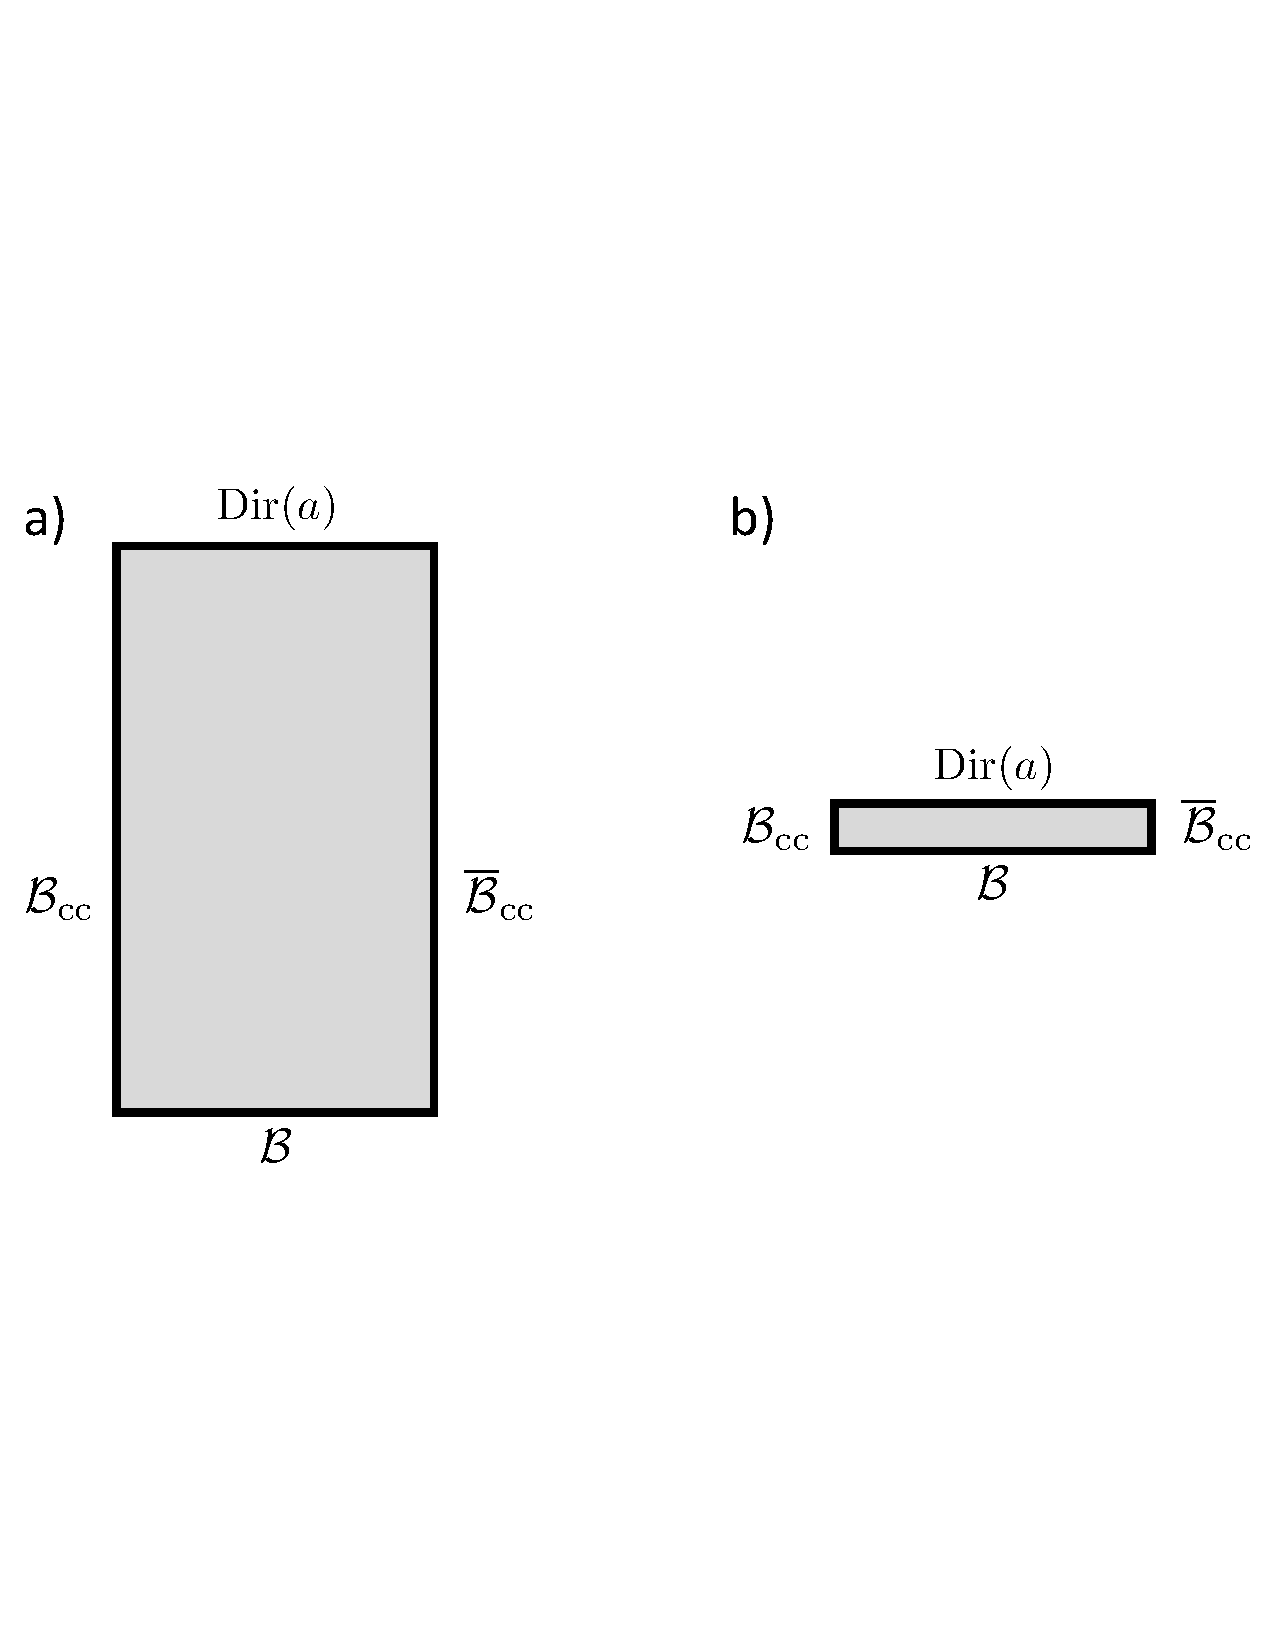
\includegraphics[width=3.2in]{Example9.pdf}
 \end{center}
\caption{\small (a) 一个矩形，底部是增广 Neumann 膜 $\B$，顶部是广义 Dirichlet 膜 $\B'$。(b) 在拓扑场论中，矩形的“高”与“宽”是任意的。在高很小的极限下，问题约化为乘积 $I\times C$ 上纯粹三维的计算。一如既往，$C$ 未画出。\label{example9}}
\end{figure} 

还有一种直接在四维中理解 (\ref{eq:ZPsi}) 的办法。这一替代视角也可以用于更一般的情形：相应的 BAA 型膜带有非平凡的 $\CP$ 丛，或者在交汇处添加了额外的手征费米子。为读出 $\Psi(a)$，我们可以把增广 Neumann 边界所产生的态 $\Psi$ 与 Dirichlet 边界条件 $\mathrm{Dir}(a)$ 所产生的态 $\Delta(a)$ 作缩并。这两个态的内积由如下路径积分表示：在图 \ref{example9}(a) 的矩形上，顶部取 $\mathrm{Dir}(a)$ 边界条件，底部取增广 Neumann 边界条件。在二维拓扑场论中，矩形的“高”与“宽”是任意的。取高远小于宽的极限（图 \ref{example9}(b)）。在此极限下，路径积分约化为 $I\times C$ 上某个三维理论的路径积分。这个三维理论来自沿区间从四维到三维的紧化，区间一端取 Dirichlet 边界条件，另一端取增广 Neumann 边界条件。这一紧化给出简单的答案，因为四维场全都被冻结在其中一个边界上：人们得到的正是当初用来构造增广 Neumann 边界条件的那个三维理论。在我们的例子里，这就是一开始那个自由超多重态的理论，只是现在把整体 $G$ 对称性与作用在 Dirichlet 边界上的 $G$ 对称性等同起来。(\ref{eq:ZPsi}) 的答案就是这个三维理论在 $I\times C $ 上的配分函数，其边界条件产生辛玻色子或其复共轭。于是，即便相应的 BAA 型膜很复杂，我们也可以绕过二维推导而直接使用 (\ref{eq:ZPsi})。在交汇处添加的任何（反）手征费米子都只贡献它们自己的配分函数，即
\begin{equation}\label{eq:ZPsifer}
\Psi(a) = \int DZ D\bar Z D\psi D\bar \psi \,e^{\int_C \left[\langle Z, \bar \partial_a Z \rangle -  \langle 
\bar Z, \partial_a \bar Z \rangle\right]+\left[( \psi, \bar \partial_a \psi ) - ( 
\bar \psi, \partial_a \bar \psi)\right]}
\end{equation} 
只要辛玻色子与费米子的合成 level 为 $-h$，这就表示 $\M(G,C)$ 上的半密度。

本节我们描述了与基本边界条件相联系的态。这一构造很容易推广，用以描述与类似的基本界面（interface）相联系的算符。基本界面的复合可以产生大量 BAA 型边界条件与界面，它们与相应算符的复合相联系。这将允许我们计算（除其他外）$C \times [0,1]$ 上 $A$-扭化三维 ${\cal N}=4$ 规范场论的配分函数，只要线段两端分别取手征与反手征边界条件。关于这一问题以及 $B$-模型中的类似问题，我们将详细分析留待将来工作。\zy{译者按（无外部依据）：本块原文有几处笔误，译文按原意译出、未改原文：§7.7 首段 “of type BAA  in  in which” 多了一个 in；§7.5 中 “correponds” 应为 “corresponds”；§7.7 中 “precisely$-h$” 缺一空格；§7.5 脚注中的 $\lmark^2$ 是源码宏，实际排为 $L^2$。}
